%% SimulacraBench Technical Report -- team TF141
%% Built from the official template (docs: simulacrabench_report_template.tex); section order unchanged.
\documentclass{article}
%% The template's [final] option leaves the footer's track name undefined; name it here.
\makeatletter\newcommand{\@trackname}{NeurIPS 2026 Competition Track: SimulacraBench.}\makeatother
\usepackage[final]{neurips_2026}

\usepackage[utf8]{inputenc}
\usepackage[T1]{fontenc}
\usepackage{hyperref}
\usepackage{url}
\usepackage{booktabs}
\usepackage{amsfonts}
\usepackage{amsmath}
\usepackage{amssymb}
\usepackage{nicefrac}
\usepackage{microtype}
\usepackage{xcolor}
\usepackage{graphicx}
\usepackage{enumitem}
\usepackage{tikz}
\usetikzlibrary{positioning,arrows.meta}

\newcommand{\teamid}{TF141}
\newcommand{\cbox}{$\square$}
\newcommand{\cboxchecked}{$\boxtimes$}
%% Placeholders that can only be filled after the test phase is scored or the repo is public.
\newcommand{\tbd}[1]{\textcolor{red}{#1}}

\title{SimulacraBench Technical Report:\\ A Self-Validating, Time-Budgeted Blend of Tabular Learners}

\author{%
  \tbd{Author name(s)}\\
  \tbd{Affiliation}\\
  \texttt{\tbd{email}}
}

\begin{document}

\maketitle

\begin{center}
\begin{tabular}{l}
\toprule
\textbf{Team ID:} \teamid \\
\bottomrule
\end{tabular}
\end{center}

\begin{abstract}
Every hidden cell is scored on its own, so the target is $P(\text{answer}\mid\text{GIVEN columns})$ for each question, estimated from the visible respondents inside the hosted run. Our submission fits five model families at run time (a shared multi-head network, a wider second network, a similarity model with learned column weights, per-question logistic regression, and the pretrained in-context learner TabICL v2) and blends them per question. Blend weights come from expectation--maximisation on held-back rows, averaged with a geometric pool. A final similarity layer is switched on per survey only when a split-half check on held-back rows shows a gain of more than two standard errors. ``Not asked'' is an ordinary answer option, and a closing step corrects for the grader's probability floor. Everything runs under one clock shared by the three surveys. Local test data were used only to choose the design. On the development leaderboard the submission scores 0.4893 (UNICEF 0.3499, World Bank 0.2335, UNHCR 0.8843). Test-phase score: \tbd{0.0000}.
\end{abstract}

%% ---------------------------------------------------------------------------
\section{Method summary}
\label{sec:method}

\subsection{Method type}
\begin{table}[h]
  \centering
  \small
  \resizebox{\linewidth}{!}{%
\begin{tabular}{@{}clcl@{}}
    \toprule
    \cbox & LLM-simulated respondents (prompting, personas) & \cbox & Fine-tuned language model \\
    \cbox & Tabular / conditional generative model & \cboxchecked & Supervised prediction (neural net, linear/GLM) \\
    \cbox & Bayesian / hierarchical / multilevel model & \cbox & Small-area estimation or post-stratification \\
    \cbox & Reweighting, raking, or calibration of the sample & \cboxchecked & Imputation / matching / nearest-neighbour \\
    \cbox & Retrieval over released or external microdata & \cbox & Agent-based or mechanistic simulation \\
    \cboxchecked & Ensemble or stacking of multiple components & \cboxchecked & Other: pretrained tabular in-context learner \\
    \bottomrule
  \end{tabular}}
\end{table}

\subsection{Pipeline}
\label{sec:pipeline}
The grader \citep{simulacrabench} scores each hidden cell by the log probability of the true answer after mixing our vector with a floor $\varepsilon=10^{-3}$, $\tilde p_k=\varepsilon+(1-K\varepsilon)p_k$. Skill is $1+\overline{\log\tilde p}/R$, with $R$ the crowd marginal's surprisal. The rule is proper \citep{gneiting2007scoring} and a hidden respondent shows only GIVEN columns, so the best prediction for a cell is the conditional distribution of its question given those columns; joint structure across questions does not matter. Our method is therefore a per-question estimator fitted inside \texttt{predict()} on the visible rows (Figure~\ref{fig:pipeline}). Visible rows go into five folds. Fold 0 (20\%), the \emph{blend fold}, is predicted by models that never saw it, and every later choice is made on it. Members then refit on all visible rows to predict the hidden ones.

\begin{figure}[h]
\centering
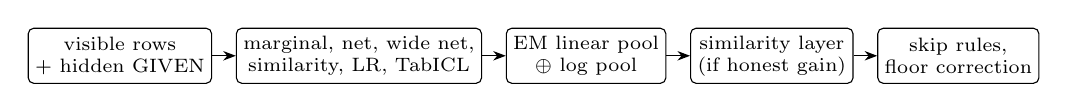
\begin{tikzpicture}[node distance=3mm, box/.style={draw, rounded corners=2pt, font=\scriptsize, align=center, inner sep=2.5pt, minimum height=7mm}, >={Stealth[length=1.6mm]}]
  \node[box] (in) {visible rows\\+ hidden GIVEN};
  \node[box, right=of in] (m) {marginal, net, wide net,\\similarity, LR, TabICL};
  \node[box, right=of m] (b) {EM linear pool\\$\oplus$ log pool};
  \node[box, right=of b] (s) {similarity layer\\(if honest gain)};
  \node[box, right=of s] (f) {skip rules,\\floor correction};
  \draw[->] (in) -- (m); \draw[->] (m) -- (b); \draw[->] (b) -- (s); \draw[->] (s) -- (f);
\end{tikzpicture}
\caption{Run-time pipeline, once per survey: members (\S\ref{sec:model}), a per-question blend of a linear and a geometric pool (\S1.6), a similarity layer kept only if an honest test supports it, exact skip rules and a floor correction (\S\ref{sec:post}).}
\label{fig:pipeline}
\end{figure}

\subsection{Inputs and feature construction}
Only the GIVEN columns and the visible PREDICT answers are used. \texttt{respondent\_id} is ignored (rows are shuffled before it is assigned), and so is question text. GIVEN columns are one-hot encoded (schema levels plus missing). TabICL instead gets two codes per column: frequency rank among context rows and schema order. For gated items the sentinel \texttt{NA\_GATED} is \emph{learned as an ordinary option}: the schemas' gate rules hold only partly (UNHCR documents 29--98\% agreement).

\subsection{Model or simulator}
\label{sec:model}
\textbf{Crowd marginal}, the fallback for every question. \textbf{Shared network}: one hidden layer (128 units) with a softmax head per question; five copies, each trained on three folds, early-stopped on a fourth and predicting the fifth, give honest out-of-fold predictions. \textbf{Wide network}: the same with two layers of 384. \textbf{Similarity model}: weight $w(x,x')=\exp(-\beta\sum_j\theta_j[x_j\neq x'_j])$, column weights $\theta$ learned by leave-one-out log loss; the votes $\sum w\,y'$ are combined with the network's prediction as a prior of pseudo-count $\alpha$, with $(\beta,\alpha)$ chosen per question. \textbf{Logistic regression} per question \citep{pedregosa2011sklearn}. \textbf{TabICL v2} \citep{qu2025tabicl,tabiclv2ckpt}, inference only: a fast pass covers every question, then rounds of two more estimators (new seed) are averaged in, up to four. Settings are in Table~\ref{tab:hyper}. Questions are treated as conditionally independent given the GIVEN columns, as the scoring rule implies.

\subsection{Fitting, training, or prompting}
All fitting happens in the hosted run on the phase's visible rows (TRAIN, then TRAIN+DEV in the test phase); we pre-train nothing. Networks use AdamW \citep{loshchilov2019adamw}, the similarity weights Adam \citep{kingma2015adam}; all selection uses held-back rows. \textbf{Clock}: \texttt{main.py} is imported once and \texttt{predict()} is called per survey under one limit, so our clock starts at import (800\,s of 900 in development, 2900\,s of 3600 in the test phase). Each survey gets a share of the time actually left, proportional to its question count, with 80\,s kept for later surveys; members stop at fixed fractions of the share, so a faster machine completes more TabICL rounds.

\subsection{Prediction and aggregation}
For question $t$ with members $m$ giving $p_m(y\mid x)$, the linear pool's weights $w_t$ maximise the blend-fold likelihood by EM \citep{dempster1977em}. They start from survey-wide weights fitted the same way over all questions, and are shrunk toward them with 40 pseudo-rows. The geometric pool $\propto\prod_m p_m^{v_{t,m}}$, $v\in[0,3]$, is fitted by L-BFGS-B with a quadratic penalty toward survey-wide exponents; its weights need not sum to one, so it can sharpen or flatten. The output is the average of the two pools. This is stacking \citep{wolpert1992stacked} with a likelihood objective.

\subsection{Post-processing and calibration}
\label{sec:post}
\textbf{Similarity layer.} The similarity model is applied once more with the blended prediction as its prior: rows with a close visible match move toward that match's answers, and other rows keep the blend. Sharpness $\beta$ is one setting per survey and the prior weight $\alpha$ is chosen per question, both on the blend fold with each row's own answers left out. Selecting on the same rows flatters the gain, so the layer is applied only if a split-half check passes: choose on one half, score on the other, swap, and require the per-row gain summed over questions to exceed $2$ standard errors. Without this check the layer lost up to 0.0012 skill on surveys lacking near-duplicates (Table~\ref{tab:gate}). \textbf{Floor correction}: for beliefs $q$, $\sum_k q_k\log(\varepsilon+(1-K\varepsilon)p_k)$ is maximised by water-filling, $\tilde p_k=\max(cq_k,\varepsilon)$; its strength is chosen per option-count group on the blend fold. \textbf{Exact skip rules} where a GIVEN-parent gate has no exception in the visible rows (rule-of-succession probabilities).

%% ---------------------------------------------------------------------------
\section{Models, data, and compute}
\label{sec:resources}

\paragraph{Pretrained models and off-the-shelf components.} One pretrained model (Table~\ref{tab:models}). Everything else is fitted at run time with PyTorch \citep{paszke2019pytorch}, scikit-learn and SciPy.

\begin{table}[h]
  \centering
  \small
  \caption{Pretrained models and off-the-shelf components.}
  \label{tab:models}
  \resizebox{\linewidth}{!}{%
\begin{tabular}{lll}
    \toprule
    Component & Version / checkpoint & Role in pipeline  \\
    \midrule
    TabICL v2 classifier & \texttt{jingang/TabICL} @ \texttt{4dcd344}, file \texttt{...-v2-20260212.ckpt} & blend member, inference only \\
    \texttt{tabicl} package & 2.2.0 (PyPI) & loads and runs the checkpoint \\
    \bottomrule
  \end{tabular}}
\end{table}

\paragraph{Data and compute.} No external data enters the submitted model. Because hosted feedback is limited to noised, rounded development scores, design choices were made offline on datasets in the competition's exact format, scored with the organisers' \texttt{score.py} (Table~\ref{tab:external}): our own generators on the three official schemas (true probabilities kept), and public surveys reshaped to the same format. Hosted: one H100, 16\,GB RAM. Locally (RTX 3050 Ti, 4\,GB) a full test-phase rehearsal of all three surveys took 2778\,s; peak memory on a 16.5k-row, 203-question survey was 3.5\,GB.

\begin{table}[h]
  \centering
  \small
  \caption{External datasets, all used \emph{only offline for model selection}; none is read by the submission.}
  \label{tab:external}
  \resizebox{\linewidth}{!}{%
\begin{tabular}{llll}
    \toprule
    Dataset & Source & Size & Use \\
    \midrule
    freeCodeCamp New Coder Survey 2016, 2021 & Kaggle (ODbL / CC-BY-SA-4.0) & 6,927 rows/sample & World-Bank-shaped tests \\
    Kaggle ML \& DS Survey 2017; Stack Overflow 2018 & Kaggle (ODbL) & 6,927 rows/sample & World-Bank-shaped tests \\
    US Current Population Survey, Jan+Feb 2024 & census.gov (public domain) & 2 months & repeat-household tests \\
    Afrobarometer Round 8 & afrobarometer.org (free, cite) & 34 countries & memory/time tests \\
    IPIP Big-Five; DASS & openpsychometrics.org & public & generic tests \\
    GVU internet survey (\texttt{kdd\_internet\_usage}) & OpenML & 10,108 & generic tests \\
    YouGov COVID-19 tracker & GitHub (research only) & 10 countries & evaluation only \\
    \bottomrule
  \end{tabular}}
\end{table}

%% ---------------------------------------------------------------------------
\section{Results}
\label{sec:results}

\subsection{Test-phase leaderboard results}
\begin{table}[h]
  \centering
  \small
  \caption{Official SimulacraBench results for team \teamid{} (skill relative to the crowd marginal). Development scores are noised and rounded by the platform.}
  \label{tab:results}
  \begin{tabular}{lrrrr}
    \toprule
    Split & Mean skill & UNICEF & World Bank & UNHCR \\
    \midrule
    Development & 0.4893 & 0.3499 & 0.2335 & 0.8843 \\
    Test        & \tbd{0.0000} & \tbd{0.0000} & \tbd{0.0000} & \tbd{0.0000} \\
    Organizer baseline (test) & \tbd{0.0000} & \tbd{0.0000} & \tbd{0.0000} & \tbd{0.0000} \\
    \bottomrule
  \end{tabular}
\end{table}

\subsection{Breakdown by population, survey, or question type}
On the development board UNICEF and UNHCR sit on the top published step and World Bank one step below (0.2335 vs.\ 0.2486). Steps are 0.015--0.02 skill, larger than most design gains, so designs were ranked locally (Table~\ref{tab:ablation}). On fabricated UNHCR-like data with known generating probabilities (development phase, 213 questions), the submission scores 0.7081 against 0.7401 for the true conditional given the GIVEN columns. The whole shortfall of 0.032 comes from rows without a near-duplicate among the visible rows (0.047, half of it on gated questions that were asked). On rows that do have one, the similarity layer brings us 0.015 \emph{above} the GIVEN-only optimum. On fabricated World Bank-like data (test-phase visibility) we are 0.0033 below the true conditional, spread evenly over all 76 questions (at most 0.00025 each), so no single question type dominates. A CatBoost member \citep{prokhorenkova2018catboost} took 16\% of the blend weight but changed real World Bank-shaped scores by $\le 0.0001$.

\begin{table}[h]
  \centering
  \small
  \caption{Local skill of successive versions (cumulative changes). DP1/DP2: development/test-phase visibility. Standard errors 0.005--0.013; differences between versions are paired, on identical cells.}
  \label{tab:ablation}
  \resizebox{\linewidth}{!}{%
\begin{tabular}{lcccccc}
    \toprule
    Version (change) & UNICEF-like & WB-like & UNHCR-like & CPS panel & fCC 2021 & Dev board \\
     & DP1 & DP1 & repeats DP1 & DP2 & DP1 & mean \\
    \midrule
    v1 logistic regression, ``not asked'' learned & 0.3410 & 0.1557 & 0.5417 & 0.2160 & 0.1955 & 0.43 \\
    v2 + network, Hamming kNN, EM blend & 0.3426 & 0.1594 & 0.6954 & 0.3741 & -- & 0.46 \\
    v3 similarity with learned weights & 0.3427 & 0.1601 & 0.7001 & 0.3987 & -- & 0.48 \\
    v5 + TabICL & 0.3442 & 0.1650 & 0.7494 & 0.4041 & -- & 0.4828 \\
    v7 + wide network & 0.3440 & 0.1646 & 0.7576 & 0.4040 & 0.2078 & 0.4828 \\
    v8 TabICL second pass & 0.3440 & 0.1655 & 0.7601 & 0.4054 & 0.2084 & -- \\
    v10 log pool, floor correction & 0.3441 & 0.1656 & 0.7632 & 0.4048 & 0.2088 & 0.4828 \\
    v12 shared clock, TabICL rounds & 0.3438 & 0.1660 & -- & 0.4055 & -- & -- \\
    v13 similarity layer (submitted) & 0.3441 & 0.1658 & 0.7659 & 0.4068 & 0.2089 & 0.4893 \\
    \bottomrule
  \end{tabular}}
\end{table}

%% ---------------------------------------------------------------------------
\section{Reproducibility}
\label{sec:repro}

\begin{itemize}[leftmargin=*,itemsep=0pt,topsep=2pt]
  \item Code: \tbd{\texttt{https://github.com/<account>/simulacrabench-tf141}} (MIT); commit \tbd{\texttt{<commit>}}. \texttt{submission/main.py} is byte-identical to the uploaded archive (SHA-256 \texttt{08bdcec2\ldots}).
  \item Rebuild the archive: \texttt{bash scripts/build\_zip.sh} (downloads the checkpoint at the pinned revision, checks its SHA-256, zips). Predictions come from the organisers' runner calling \texttt{predict()}; locally \texttt{python starter-kit/score.py --submission submission --data <dir> --phase 2}.
  \item Environment: Python 3.13, versions pinned in \texttt{requirements-dev.txt}; organisers' starter kit as a submodule at \texttt{aa03186}. Weights: TabICL v2, public (BSD-3-Clause), pinned by revision and checksum.
  \item Seeds are fixed, but the number of TabICL rounds depends on machine speed and survey order; \texttt{SB\_FULL\_PASSES} and \texttt{SB\_CLOCK\_SECONDS} pin it.
\end{itemize}

%% ---------------------------------------------------------------------------
\section{Limitations}
\label{sec:limitations}

The method only estimates per-cell conditional distributions. It makes no claim about joint answer patterns, so samples drawn from it would not be coherent simulated respondents. Its gains over a strong single learner are small (Table~\ref{tab:ablation}) and were measured on proxy data. The similarity layer helps only where visible rows contain near-duplicate profiles, and the split-half gate decides that per run. With few visible rows per GIVEN profile, scores for rare subgroups rest mostly on the marginal and should not be read as subgroup estimates.

%% ---------------------------------------------------------------------------
\bibliographystyle{plainnat}
\bibliography{refs}

%% ---------------------------------------------------------------------------
\clearpage
\appendix

\section{Full configuration}
Everything below is in \texttt{submission/main.py}; no prompts are used.

\begin{table}[h]
\centering
\small
\caption{Hyperparameters and selection rules. ``Blend fold'': the 20\% of visible rows (fold 0, seed 0) held back for every choice.}
\label{tab:hyper}
\begin{tabular}{p{2.6cm}p{10.4cm}}
\toprule
Component & Setting \\
\midrule
Encoding & One-hot of every GIVEN level plus a missing level. TabICL: frequency rank among context rows and schema order, per column. \\
Marginal & Counts $+0.5$ per option (sentinel included). \\
Shared network & 128 ReLU, dropout 0.5; heads per question; output bias $=\log$ marginal; AdamW, lr $3\cdot10^{-3}$, wd $10^{-2}$ (none on output bias), batch 512, $\le$80 epochs, patience 10; 5 nets (train 3 folds, stop 1, predict 1); per-question best-epoch snapshot. Deadline $0.15$ of the survey budget. \\
Wide network & As above with $384\times384$, dropout 0.15. Deadline $0.30$. \\
Similarity model & $w=\exp(-\beta\sum_j\theta_j[x_j\ne x'_j])$; $\log\theta$ by Adam (lr 0.08, $\le$300 steps of 512 rows, clamp $[-6,3]$, early stop on 1024 probe rows), leave-one-out loss; $\beta\in\{0.5,1,2,4\}$, $\alpha\in\{0.05,0.5,5\}$ per question by leave-one-out loss; prior = shared network. Deadlines 0.37 (weights), 0.48 (votes). \\
Logistic regression & scikit-learn \texttt{LogisticRegression}, $C\in\{0.03,0.3,3,30\}$ on the blend fold, refit on all rows; questions in order of decreasing marginal entropy. Deadline 0.84. \\
TabICL v2 & Pass 0: rank encoding, 1 estimator, seed 0, all questions (deadline 0.70). Rounds 1--4: both encodings, 2 estimators, \texttt{norm\_methods=none}, temperature 1, seed $=$ round$-1$, averaged; deadline 0.94. \\
Linear pool & Survey-wide weights by EM (300 iterations); per question EM (400 iterations) with 40 prior pseudo-rows toward them. \\
Log pool & Exponents in $[0,3]$, L-BFGS-B; survey-wide fit, then per question with penalty $s\lVert v-g\rVert^2$, $s=\mathrm{clip}(2000/n_\text{blend},1,4)$. Output $=0.5\cdot$linear$+0.5\cdot$log. \\
Similarity layer & $\beta\in\{0.25,\dots,8\}$ (6 values) per survey; $\alpha\in\{0.03,\dots,30\}$ (7 values) per question; question kept if blend-fold loss drops by $>3\cdot10^{-4}$ nats; split-half (seed 7) honest gain $>2$ SE. \\
Floor correction & Strength $\{0,0.5,1,1.5\}\varepsilon$ per option-count group (2--3, 4--6, 7--10, 11+), on the blend fold. \\
Skip rules & GIVEN parent, no exception in visible rows, $\ge$20 rows each side; sentinel $1/(n+2)$ or $1-1/(n+2)$. \\
Clock & From import: 800\,s (dev) / 2900\,s (test); budget $=$ (time left $-$ 80\,s) $\times$ share of the 301 questions; last survey takes all that is left. Phase detected from the number of hidden rows. \\
\bottomrule
\end{tabular}
\end{table}

\section{Additional results}

\begin{table}[h]
\centering
\small
\caption{The similarity layer's split-half gate (development-phase visibility unless noted). ``Permissive'': applied whenever any question improved on the blend fold.}
\label{tab:gate}
\resizebox{\linewidth}{!}{%
\begin{tabular}{lcccc}
\toprule
Dataset & Without layer & Permissive & Gated (submitted) & Gate decision (gain / SE) \\
\midrule
GVU proxy with repeats & 0.1558 & 0.1546 & 0.1558 & off \\
GVU proxy & 0.1123 & 0.1118 & 0.1123 & off \\
World Bank-like & 0.1658 & 0.1655 & 0.1658 & off \\
fCC 2021 (World Bank-shaped) & 0.2089 & 0.2089 & 0.2089 & off \\
UNHCR-like, repeats & 0.7632$^\ast$ & 0.7660 & 0.7659 & on (2.6) \\
CPS panel (test-phase visibility) & 0.4055$^\ast$ & 0.4068 & 0.4068 & on (2.2) \\
\bottomrule
\end{tabular}}

\smallskip\footnotesize $^\ast$ previous version (v10 and v12 respectively) rather than v13 with the layer switched off.
\end{table}

\paragraph{Ideas that did not help locally.} Several similarity kernels, ordinal smoothing of ordered answers, ordered copies of GIVEN columns, a two-part (asked / answer) logistic model, and CatBoost as an extra member. Extra TabICL estimators help only slightly (at most $+0.0006$ on World Bank-like data), which is why they are added in rounds only while time remains. Development uploads of the same design with more run time (850\,s) returned the same or a lower rounded score, consistent with the rounding step exceeding the effect.

\end{document}
